\begin{figure}[!htbp]
\centering
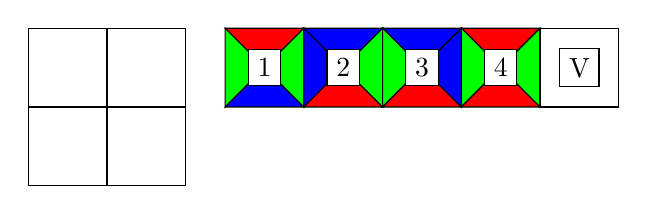
\begin{tikzpicture}

\draw (0,0) grid (2,2);

\draw[fill=red] (0 + 2.5, 0 + 2) -- (0 + 3.5, 0 + 2) -- (0 + 3, 0 + 1.5) -- cycle;
\draw[fill=green] (0 + 2.5, 0 + 2) -- (0 + 2.5, 0 + 1) -- (0 + 3, 0 + 1.5) -- cycle;
\draw[fill=blue] (0 + 2.5, 0 + 1) -- (0 + 3.5, 0 + 1) -- (0 + 3, 0 + 1.5) -- cycle;
\draw[fill=green] (0 + 3.5, 0 + 1) -- (0 + 3.5, 0 + 2) -- (0 + 3, 0 + 1.5) -- cycle;
\node[draw, fill=white] at (0 + 3, 0 + 1.5) {1};

\draw[fill=blue] (1 + 2.5, 0 + 2) -- (1 + 3.5, 0 + 2) -- (1 + 3, 0 + 1.5) -- cycle;
\draw[fill=blue] (1 + 2.5, 0 + 2) -- (1 + 2.5, 0 + 1) -- (1 + 3, 0 + 1.5) -- cycle;
\draw[fill=red] (1 + 2.5, 0 + 1) -- (1 + 3.5, 0 + 1) -- (1 + 3, 0 + 1.5) -- cycle;
\draw[fill=green] (1 + 3.5, 0 + 1) -- (1 + 3.5, 0 + 2) -- (1 + 3, 0 + 1.5) -- cycle;
\node[draw, fill=white] at (1 + 3, 0 + 1.5) {2};

\draw[fill=blue] (2 + 2.5, 0 + 2) -- (2 + 3.5, 0 + 2) -- (2 + 3, 0 + 1.5) -- cycle;
\draw[fill=green] (2 + 2.5, 0 + 2) -- (2 + 2.5, 0 + 1) -- (2 + 3, 0 + 1.5) -- cycle;
\draw[fill=red] (2 + 2.5, 0 + 1) -- (2 + 3.5, 0 + 1) -- (2 + 3, 0 + 1.5) -- cycle;
\draw[fill=blue] (2 + 3.5, 0 + 1) -- (2 + 3.5, 0 + 2) -- (2 + 3, 0 + 1.5) -- cycle;
\node[draw, fill=white] at (2 + 3, 0 + 1.5) {3};

\draw[fill=red] (3 + 2.5, 0 + 2) -- (3 + 3.5, 0 + 2) -- (3 + 3, 0 + 1.5) -- cycle;
\draw[fill=green] (3 + 2.5, 0 + 2) -- (3 + 2.5, 0 + 1) -- (3 + 3, 0 + 1.5) -- cycle;
\draw[fill=red] (3 + 2.5, 0 + 1) -- (3 + 3.5, 0 + 1) -- (3 + 3, 0 + 1.5) -- cycle;
\draw[fill=green] (3 + 3.5, 0 + 1) -- (3 + 3.5, 0 + 2) -- (3 + 3, 0 + 1.5) -- cycle;
\node[draw, fill=white] at (3 + 3, 0 + 1.5) {4};

\draw[black] (4 + 2.5, 0 + 2) rectangle (5 + 2.5, 1);
\node[draw, fill=white] at (4 + 3, 0 + 1.5) {V};

\end{tikzpicture}

\caption{Tablero y fichas de entrada. La ficha \emph{V} va a representar dejar el casillero vac\'io}
\label{ej_3:entrada}
\end{figure}

\begin{figure}[!htbp]
\centering
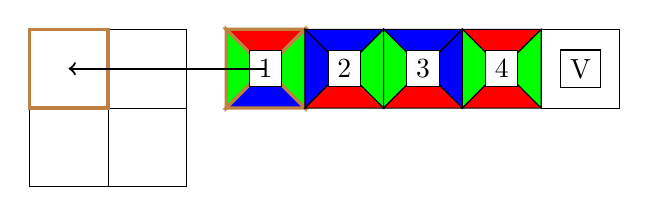
\begin{tikzpicture}

\draw (0,0) grid (2,2);

\draw[brown,very thick] (0,2) rectangle (1,1);

\draw[brown,very thick,fill=red] (0 + 2.5, 0 + 2) -- (0 + 3.5, 0 + 2) -- (0 + 3, 0 + 1.5) -- cycle;
\draw[brown,very thick,fill=green] (0 + 2.5, 0 + 2) -- (0 + 2.5, 0 + 1) -- (0 + 3, 0 + 1.5) -- cycle;
\draw[brown,very thick,fill=blue] (0 + 2.5, 0 + 1) -- (0 + 3.5, 0 + 1) -- (0 + 3, 0 + 1.5) -- cycle;
\draw[brown,very thick,fill=green] (0 + 3.5, 0 + 1) -- (0 + 3.5, 0 + 2) -- (0 + 3, 0 + 1.5) -- cycle;
\node[draw, fill=white] at (0 + 3, 0 + 1.5) {1};

\draw[->,thick] (0 + 3, 0 + 1.5) -- (0 + 0.5, 0 + 1.5);

\draw[fill=blue] (1 + 2.5, 0 + 2) -- (1 + 3.5, 0 + 2) -- (1 + 3, 0 + 1.5) -- cycle;
\draw[fill=blue] (1 + 2.5, 0 + 2) -- (1 + 2.5, 0 + 1) -- (1 + 3, 0 + 1.5) -- cycle;
\draw[fill=red] (1 + 2.5, 0 + 1) -- (1 + 3.5, 0 + 1) -- (1 + 3, 0 + 1.5) -- cycle;
\draw[fill=green] (1 + 3.5, 0 + 1) -- (1 + 3.5, 0 + 2) -- (1 + 3, 0 + 1.5) -- cycle;
\node[draw, fill=white] at (1 + 3, 0 + 1.5) {2};

\draw[fill=blue] (2 + 2.5, 0 + 2) -- (2 + 3.5, 0 + 2) -- (2 + 3, 0 + 1.5) -- cycle;
\draw[fill=green] (2 + 2.5, 0 + 2) -- (2 + 2.5, 0 + 1) -- (2 + 3, 0 + 1.5) -- cycle;
\draw[fill=red] (2 + 2.5, 0 + 1) -- (2 + 3.5, 0 + 1) -- (2 + 3, 0 + 1.5) -- cycle;
\draw[fill=blue] (2 + 3.5, 0 + 1) -- (2 + 3.5, 0 + 2) -- (2 + 3, 0 + 1.5) -- cycle;
\node[draw, fill=white] at (2 + 3, 0 + 1.5) {3};

\draw[fill=red] (3 + 2.5, 0 + 2) -- (3 + 3.5, 0 + 2) -- (3 + 3, 0 + 1.5) -- cycle;
\draw[fill=green] (3 + 2.5, 0 + 2) -- (3 + 2.5, 0 + 1) -- (3 + 3, 0 + 1.5) -- cycle;
\draw[fill=red] (3 + 2.5, 0 + 1) -- (3 + 3.5, 0 + 1) -- (3 + 3, 0 + 1.5) -- cycle;
\draw[fill=green] (3 + 3.5, 0 + 1) -- (3 + 3.5, 0 + 2) -- (3 + 3, 0 + 1.5) -- cycle;
\node[draw, fill=white] at (3 + 3, 0 + 1.5) {4};

\draw[black] (4 + 2.5, 0 + 2) rectangle (5 + 2.5, 1);
\node[draw, fill=white] at (4 + 3, 0 + 1.5) {V};

\end{tikzpicture}

\caption{Comienza con la primer posici\'on del tablero y la primera ficha disponible para colocar, siendo esta v\'alida para ser colocada}
\label{ej_3:primera}
\end{figure}

\begin{figure}[!htbp]
\centering
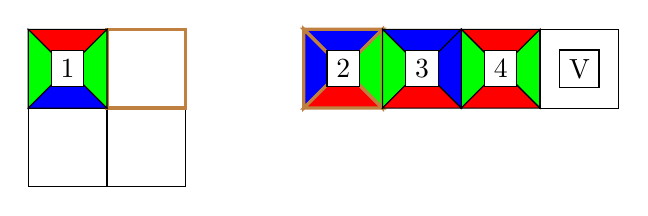
\begin{tikzpicture}

\draw (0,0) grid (2,2);

\draw[brown,very thick] (1,2) rectangle (2,1);

\draw[fill=red] (0 + 0, 0 + 2) -- (0 + 1, 0 + 2) -- (0 + 0.5, 0 + 1.5) -- cycle;
\draw[fill=green] (0 + 0, 0 + 2) -- (0 + 0, 0 + 1) -- (0 + 0.5, 0 + 1.5) -- cycle;
\draw[fill=blue] (0 + 0, 0 + 1) -- (0 + 1, 0 + 1) -- (0 + 0.5, 0 + 1.5) -- cycle;
\draw[fill=green] (0 + 1, 0 + 1) -- (0 + 1, 0 + 2) -- (0 + 0.5, 0 + 1.5) -- cycle;
\node[draw, fill=white] at (0 + 0.5, 0 + 1.5) {1};

\draw[brown,very thick,fill=blue] (1 + 2.5, 0 + 2) -- (1 + 3.5, 0 + 2) -- (1 + 3, 0 + 1.5) -- cycle;
\draw[brown,very thick,fill=blue] (1 + 2.5, 0 + 2) -- (1 + 2.5, 0 + 1) -- (1 + 3, 0 + 1.5) -- cycle;
\draw[brown,very thick,fill=red] (1 + 2.5, 0 + 1) -- (1 + 3.5, 0 + 1) -- (1 + 3, 0 + 1.5) -- cycle;
\draw[brown,very thick,fill=green] (1 + 3.5, 0 + 1) -- (1 + 3.5, 0 + 2) -- (1 + 3, 0 + 1.5) -- cycle;
\node[draw, fill=white] at (1 + 3, 0 + 1.5) {2};

\draw[fill=blue] (2 + 2.5, 0 + 2) -- (2 + 3.5, 0 + 2) -- (2 + 3, 0 + 1.5) -- cycle;
\draw[fill=green] (2 + 2.5, 0 + 2) -- (2 + 2.5, 0 + 1) -- (2 + 3, 0 + 1.5) -- cycle;
\draw[fill=red] (2 + 2.5, 0 + 1) -- (2 + 3.5, 0 + 1) -- (2 + 3, 0 + 1.5) -- cycle;
\draw[fill=blue] (2 + 3.5, 0 + 1) -- (2 + 3.5, 0 + 2) -- (2 + 3, 0 + 1.5) -- cycle;
\node[draw, fill=white] at (2 + 3, 0 + 1.5) {3};

\draw[fill=red] (3 + 2.5, 0 + 2) -- (3 + 3.5, 0 + 2) -- (3 + 3, 0 + 1.5) -- cycle;
\draw[fill=green] (3 + 2.5, 0 + 2) -- (3 + 2.5, 0 + 1) -- (3 + 3, 0 + 1.5) -- cycle;
\draw[fill=red] (3 + 2.5, 0 + 1) -- (3 + 3.5, 0 + 1) -- (3 + 3, 0 + 1.5) -- cycle;
\draw[fill=green] (3 + 3.5, 0 + 1) -- (3 + 3.5, 0 + 2) -- (3 + 3, 0 + 1.5) -- cycle;
\node[draw, fill=white] at (3 + 3, 0 + 1.5) {4};

\draw[black] (4 + 2.5, 0 + 2) rectangle (5 + 2.5, 1);
\node[draw, fill=white] at (4 + 3, 0 + 1.5) {V};

\end{tikzpicture}

\caption{Se mueve a la segunda posici\'on el tablero y analiza la primer ficha disponible, pero no es v\'alida su colocaci\'on}
\label{ej_3:segunda}
\end{figure}

\begin{figure}[!htbp]
\centering
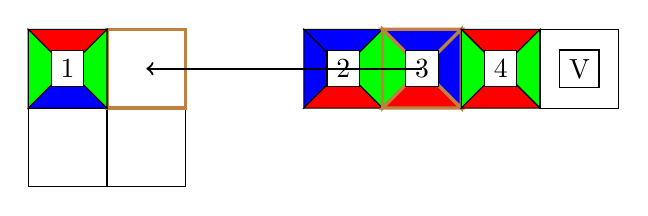
\begin{tikzpicture}

\draw (0,0) grid (2,2);

\draw[brown,very thick] (1,2) rectangle (2,1);

\draw[fill=red] (0 + 0, 0 + 2) -- (0 + 1, 0 + 2) -- (0 + 0.5, 0 + 1.5) -- cycle;
\draw[fill=green] (0 + 0, 0 + 2) -- (0 + 0, 0 + 1) -- (0 + 0.5, 0 + 1.5) -- cycle;
\draw[fill=blue] (0 + 0, 0 + 1) -- (0 + 1, 0 + 1) -- (0 + 0.5, 0 + 1.5) -- cycle;
\draw[fill=green] (0 + 1, 0 + 1) -- (0 + 1, 0 + 2) -- (0 + 0.5, 0 + 1.5) -- cycle;
\node[draw, fill=white] at (0 + 0.5, 0 + 1.5) {1};

\draw[fill=blue] (1 + 2.5, 0 + 2) -- (1 + 3.5, 0 + 2) -- (1 + 3, 0 + 1.5) -- cycle;
\draw[fill=blue] (1 + 2.5, 0 + 2) -- (1 + 2.5, 0 + 1) -- (1 + 3, 0 + 1.5) -- cycle;
\draw[fill=red] (1 + 2.5, 0 + 1) -- (1 + 3.5, 0 + 1) -- (1 + 3, 0 + 1.5) -- cycle;
\draw[fill=green] (1 + 3.5, 0 + 1) -- (1 + 3.5, 0 + 2) -- (1 + 3, 0 + 1.5) -- cycle;
\node[draw, fill=white] at (1 + 3, 0 + 1.5) {2};

\draw[brown,very thick,fill=blue] (2 + 2.5, 0 + 2) -- (2 + 3.5, 0 + 2) -- (2 + 3, 0 + 1.5) -- cycle;
\draw[brown,very thick,fill=green] (2 + 2.5, 0 + 2) -- (2 + 2.5, 0 + 1) -- (2 + 3, 0 + 1.5) -- cycle;
\draw[brown,very thick,fill=red] (2 + 2.5, 0 + 1) -- (2 + 3.5, 0 + 1) -- (2 + 3, 0 + 1.5) -- cycle;
\draw[brown,very thick,fill=blue] (2 + 3.5, 0 + 1) -- (2 + 3.5, 0 + 2) -- (2 + 3, 0 + 1.5) -- cycle;
\node[draw, fill=white] at (2 + 3, 0 + 1.5) {3};

\draw[->,thick] (0 + 5, 0 + 1.5) -- (0 + 1.5, 0 + 1.5);

\draw[fill=red] (3 + 2.5, 0 + 2) -- (3 + 3.5, 0 + 2) -- (3 + 3, 0 + 1.5) -- cycle;
\draw[fill=green] (3 + 2.5, 0 + 2) -- (3 + 2.5, 0 + 1) -- (3 + 3, 0 + 1.5) -- cycle;
\draw[fill=red] (3 + 2.5, 0 + 1) -- (3 + 3.5, 0 + 1) -- (3 + 3, 0 + 1.5) -- cycle;
\draw[fill=green] (3 + 3.5, 0 + 1) -- (3 + 3.5, 0 + 2) -- (3 + 3, 0 + 1.5) -- cycle;
\node[draw, fill=white] at (3 + 3, 0 + 1.5) {4};

\draw[black] (4 + 2.5, 0 + 2) rectangle (5 + 2.5, 1);
\node[draw, fill=white] at (4 + 3, 0 + 1.5) {V};

\end{tikzpicture}

\caption{Ahora analiza la ficha n\'umero 3, la cual si es v\'alida colocar}
\label{ej_3:segunda_valida}
\end{figure}

\begin{figure}[!htbp]
\centering
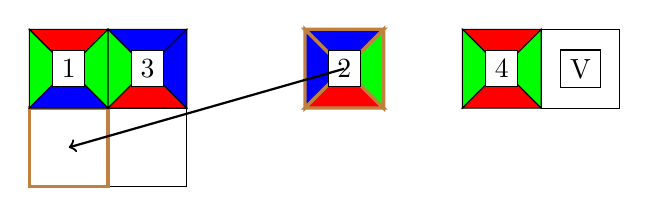
\begin{tikzpicture}

\draw (0,0) grid (2,2);

\draw[brown,very thick] (0,1) rectangle (1,0);

\draw[fill=red] (0 + 0, 0 + 2) -- (0 + 1, 0 + 2) -- (0 + 0.5, 0 + 1.5) -- cycle;
\draw[fill=green] (0 + 0, 0 + 2) -- (0 + 0, 0 + 1) -- (0 + 0.5, 0 + 1.5) -- cycle;
\draw[fill=blue] (0 + 0, 0 + 1) -- (0 + 1, 0 + 1) -- (0 + 0.5, 0 + 1.5) -- cycle;
\draw[fill=green] (0 + 1, 0 + 1) -- (0 + 1, 0 + 2) -- (0 + 0.5, 0 + 1.5) -- cycle;
\node[draw, fill=white] at (0 + 0.5, 1 + 0.5) {1};

\draw[brown,very thick,fill=blue] (1 + 2.5, 0 + 2) -- (1 + 3.5, 0 + 2) -- (1 + 3, 0 + 1.5) -- cycle;
\draw[brown,very thick,fill=blue] (1 + 2.5, 0 + 2) -- (1 + 2.5, 0 + 1) -- (1 + 3, 0 + 1.5) -- cycle;
\draw[brown,very thick,fill=red] (1 + 2.5, 0 + 1) -- (1 + 3.5, 0 + 1) -- (1 + 3, 0 + 1.5) -- cycle;
\draw[brown,very thick,fill=green] (1 + 3.5, 0 + 1) -- (1 + 3.5, 0 + 2) -- (1 + 3, 0 + 1.5) -- cycle;
\node[draw, fill=white] at (1 + 3, 0 + 1.5) {2};

\draw[->,thick] (0 + 4, 0 + 1.5) -- (0 + 0.5, 0 + 0.5);

\draw[fill=blue] (1 + 0, 0 + 2) -- (1 + 1, 0 + 2) -- (1 + 0.5, 0 + 1.5) -- cycle;
\draw[fill=green] (1 + 0, 0 + 2) -- (1 + 0, 0 + 1) -- (1 + 0.5, 0 + 1.5) -- cycle;
\draw[fill=red] (1 + 0, 0 + 1) -- (1 + 1, 0 + 1) -- (1 + 0.5, 0 + 1.5) -- cycle;
\draw[fill=blue] (1 + 1, 0 + 1) -- (1 + 1, 0 + 2) -- (1 + 0.5, 0 + 1.5) -- cycle;
\node[draw, fill=white] at (1 + 0.5, 1 + 0.5) {3};

\draw[fill=red] (3 + 2.5, 0 + 2) -- (3 + 3.5, 0 + 2) -- (3 + 3, 0 + 1.5) -- cycle;
\draw[fill=green] (3 + 2.5, 0 + 2) -- (3 + 2.5, 0 + 1) -- (3 + 3, 0 + 1.5) -- cycle;
\draw[fill=red] (3 + 2.5, 0 + 1) -- (3 + 3.5, 0 + 1) -- (3 + 3, 0 + 1.5) -- cycle;
\draw[fill=green] (3 + 3.5, 0 + 1) -- (3 + 3.5, 0 + 2) -- (3 + 3, 0 + 1.5) -- cycle;
\node[draw, fill=white] at (3 + 3, 0 + 1.5) {4};

\draw[black] (4 + 2.5, 0 + 2) rectangle (5 + 2.5, 1);
\node[draw, fill=white] at (4 + 3, 0 + 1.5) {V};

\end{tikzpicture}

\caption{Avanza al siguiente casillero y vuelve a fijarse en la segunda ficha disponible para poner, como es v\'alida, la coloca}
\label{ej_3:ante_ultima}
\end{figure}

\begin{figure}[!htbp]
\centering
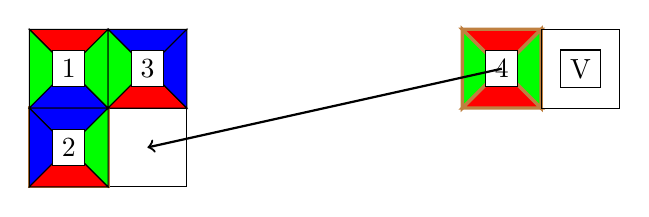
\begin{tikzpicture}

\draw (0,0) grid (2,2);

\draw[brown,very thick] (0,1) rectangle (1,0);

\draw[fill=red] (0 + 0, 0 + 2) -- (0 + 1, 0 + 2) -- (0 + 0.5, 0 + 1.5) -- cycle;
\draw[fill=green] (0 + 0, 0 + 2) -- (0 + 0, 0 + 1) -- (0 + 0.5, 0 + 1.5) -- cycle;
\draw[fill=blue] (0 + 0, 0 + 1) -- (0 + 1, 0 + 1) -- (0 + 0.5, 0 + 1.5) -- cycle;
\draw[fill=green] (0 + 1, 0 + 1) -- (0 + 1, 0 + 2) -- (0 + 0.5, 0 + 1.5) -- cycle;
\node[draw, fill=white] at (0 + 0.5, 1 + 0.5) {1};

\draw[fill=blue] (0 + 0, 0 + 1) -- (0 + 1, 0 + 1) -- (0 + 0.5, 0 + 0.5) -- cycle;
\draw[fill=blue] (0 + 0, 0 + 1) -- (0 + 0, 0 + 0) -- (0 + 0.5, 0 + 0.5) -- cycle;
\draw[fill=red]  (0 + 0, 0 + 0) -- (0 + 1, 0 + 0) -- (0 + 0.5, 0 + 0.5) -- cycle;
\draw[fill=green] (0 + 1, 0 + 0) -- (0 + 1, 0 + 1) -- (0 + 0.5, 0 + 0.5) -- cycle;
\node[draw, fill=white] at (0 + 0.5, 0 + 0.5) {2};

\draw[fill=blue] (1 + 0, 0 + 2) -- (1 + 1, 0 + 2) -- (1 + 0.5, 0 + 1.5) -- cycle;
\draw[fill=green] (1 + 0, 0 + 2) -- (1 + 0, 0 + 1) -- (1 + 0.5, 0 + 1.5) -- cycle;
\draw[fill=red] (1 + 0, 0 + 1) -- (1 + 1, 0 + 1) -- (1 + 0.5, 0 + 1.5) -- cycle;
\draw[fill=blue] (1 + 1, 0 + 1) -- (1 + 1, 0 + 2) -- (1 + 0.5, 0 + 1.5) -- cycle;
\node[draw, fill=white] at (1 + 0.5, 1 + 0.5) {3};

\draw[brown,very thick,fill=red] (3 + 2.5, 0 + 2) -- (3 + 3.5, 0 + 2) -- (3 + 3, 0 + 1.5) -- cycle;
\draw[brown,very thick,fill=green] (3 + 2.5, 0 + 2) -- (3 + 2.5, 0 + 1) -- (3 + 3, 0 + 1.5) -- cycle;
\draw[brown,very thick,fill=red] (3 + 2.5, 0 + 1) -- (3 + 3.5, 0 + 1) -- (3 + 3, 0 + 1.5) -- cycle;
\draw[brown,very thick,fill=green] (3 + 3.5, 0 + 1) -- (3 + 3.5, 0 + 2) -- (3 + 3, 0 + 1.5) -- cycle;
\node[draw, fill=white] at (3 + 3, 0 + 1.5) {4};

\draw[->,thick] (0 + 6, 0 + 1.5) -- (0 + 1.5, 0 + 0.5);

\draw[black] (4 + 2.5, 0 + 2) rectangle (5 + 2.5, 1);
\node[draw, fill=white] at (4 + 3, 0 + 1.5) {V};

\end{tikzpicture}

\caption{Avanza al \'ultimo casillero y se fija en la \'ultima ficha disponible que queda, como es v\'alida, la coloca}
\label{ej_3:ultima_ficha}
\end{figure}

\begin{figure}[!htbp]
\centering
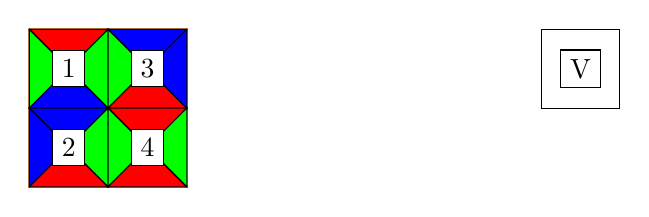
\begin{tikzpicture}

\draw[brown,very thick] (0,0) grid (2,2);

\draw[fill=red] (0 + 0, 0 + 2) -- (0 + 1, 0 + 2) -- (0 + 0.5, 0 + 1.5) -- cycle;
\draw[fill=green] (0 + 0, 0 + 2) -- (0 + 0, 0 + 1) -- (0 + 0.5, 0 + 1.5) -- cycle;
\draw[fill=blue] (0 + 0, 0 + 1) -- (0 + 1, 0 + 1) -- (0 + 0.5, 0 + 1.5) -- cycle;
\draw[fill=green] (0 + 1, 0 + 1) -- (0 + 1, 0 + 2) -- (0 + 0.5, 0 + 1.5) -- cycle;
\node[draw, fill=white] at (0 + 0.5, 1 + 0.5) {1};

\draw[fill=blue] (0 + 0, 0 + 1) -- (0 + 1, 0 + 1) -- (0 + 0.5, 0 + 0.5) -- cycle;
\draw[fill=blue] (0 + 0, 0 + 1) -- (0 + 0, 0 + 0) -- (0 + 0.5, 0 + 0.5) -- cycle;
\draw[fill=red]  (0 + 0, 0 + 0) -- (0 + 1, 0 + 0) -- (0 + 0.5, 0 + 0.5) -- cycle;
\draw[fill=green] (0 + 1, 0 + 0) -- (0 + 1, 0 + 1) -- (0 + 0.5, 0 + 0.5) -- cycle;
\node[draw, fill=white] at (0 + 0.5, 0 + 0.5) {2};

\draw[fill=blue] (1 + 0, 0 + 2) -- (1 + 1, 0 + 2) -- (1 + 0.5, 0 + 1.5) -- cycle;
\draw[fill=green] (1 + 0, 0 + 2) -- (1 + 0, 0 + 1) -- (1 + 0.5, 0 + 1.5) -- cycle;
\draw[fill=red] (1 + 0, 0 + 1) -- (1 + 1, 0 + 1) -- (1 + 0.5, 0 + 1.5) -- cycle;
\draw[fill=blue] (1 + 1, 0 + 1) -- (1 + 1, 0 + 2) -- (1 + 0.5, 0 + 1.5) -- cycle;
\node[draw, fill=white] at (1 + 0.5, 1 + 0.5) {3};

\draw[fill=red]  (1 + 0, 0 + 1) -- (1 + 1, 0 + 1) -- (1 + 0.5, 0 + 0.5) -- cycle;
\draw[fill=green] (1 + 0, 0 + 1) -- (1 + 0, 0 + 0) -- (1 + 0.5, 0 + 0.5) -- cycle;
\draw[fill=red] (1 + 0, 0 + 0) -- (1 + 1, 0 + 0) -- (1 + 0.5, 0 + 0.5) -- cycle;
\draw[fill=green] (1 + 1, 0 + 0) -- (1 + 1, 0 + 1) -- (1 + 0.5, 0 + 0.5) -- cycle;
\node[draw, fill=white] at (1 + 0.5, 0 + 0.5) {4};

\draw[black] (4 + 2.5, 0 + 2) rectangle (5 + 2.5, 1);
\node[draw, fill=white] at (4 + 3, 0 + 1.5) {V};

\end{tikzpicture}

\caption{Al no quedar casillero sin procesar, se llega al caso base y guarda la combinaci\'on como la m\'axima encontrada}
\label{ej_3:caso_base}
\end{figure}

\begin{figure}[!htbp]
\centering
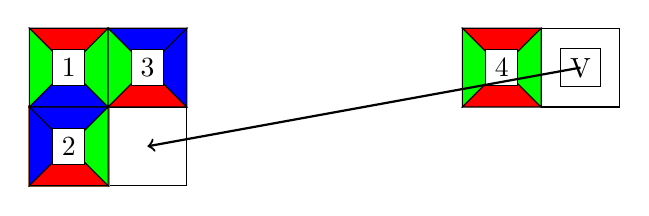
\begin{tikzpicture}

\draw (0,0) grid (2,2);

\draw[brown,very thick] (0,1) rectangle (1,0);

\draw[fill=red] (0 + 0, 0 + 2) -- (0 + 1, 0 + 2) -- (0 + 0.5, 0 + 1.5) -- cycle;
\draw[fill=green] (0 + 0, 0 + 2) -- (0 + 0, 0 + 1) -- (0 + 0.5, 0 + 1.5) -- cycle;
\draw[fill=blue] (0 + 0, 0 + 1) -- (0 + 1, 0 + 1) -- (0 + 0.5, 0 + 1.5) -- cycle;
\draw[fill=green] (0 + 1, 0 + 1) -- (0 + 1, 0 + 2) -- (0 + 0.5, 0 + 1.5) -- cycle;
\node[draw, fill=white] at (0 + 0.5, 1 + 0.5) {1};

\draw[fill=blue] (0 + 0, 0 + 1) -- (0 + 1, 0 + 1) -- (0 + 0.5, 0 + 0.5) -- cycle;
\draw[fill=blue] (0 + 0, 0 + 1) -- (0 + 0, 0 + 0) -- (0 + 0.5, 0 + 0.5) -- cycle;
\draw[fill=red]  (0 + 0, 0 + 0) -- (0 + 1, 0 + 0) -- (0 + 0.5, 0 + 0.5) -- cycle;
\draw[fill=green] (0 + 1, 0 + 0) -- (0 + 1, 0 + 1) -- (0 + 0.5, 0 + 0.5) -- cycle;
\node[draw, fill=white] at (0 + 0.5, 0 + 0.5) {2};

\draw[fill=blue] (1 + 0, 0 + 2) -- (1 + 1, 0 + 2) -- (1 + 0.5, 0 + 1.5) -- cycle;
\draw[fill=green] (1 + 0, 0 + 2) -- (1 + 0, 0 + 1) -- (1 + 0.5, 0 + 1.5) -- cycle;
\draw[fill=red] (1 + 0, 0 + 1) -- (1 + 1, 0 + 1) -- (1 + 0.5, 0 + 1.5) -- cycle;
\draw[fill=blue] (1 + 1, 0 + 1) -- (1 + 1, 0 + 2) -- (1 + 0.5, 0 + 1.5) -- cycle;
\node[draw, fill=white] at (1 + 0.5, 1 + 0.5) {3};

\draw[fill=red] (3 + 2.5, 0 + 2) -- (3 + 3.5, 0 + 2) -- (3 + 3, 0 + 1.5) -- cycle;
\draw[fill=green] (3 + 2.5, 0 + 2) -- (3 + 2.5, 0 + 1) -- (3 + 3, 0 + 1.5) -- cycle;
\draw[fill=red] (3 + 2.5, 0 + 1) -- (3 + 3.5, 0 + 1) -- (3 + 3, 0 + 1.5) -- cycle;
\draw[fill=green] (3 + 3.5, 0 + 1) -- (3 + 3.5, 0 + 2) -- (3 + 3, 0 + 1.5) -- cycle;
\node[draw, fill=white] at (3 + 3, 0 + 1.5) {4};


\draw[black] (4 + 2.5, 0 + 2) rectangle (5 + 2.5, 1);
\node[draw, fill=white] at (4 + 3, 0 + 1.5) {V};

\draw[->,thick] (0 + 7, 0 + 1.5) -- (1 + 0.5, 0 + 0.5);

\end{tikzpicture}

\caption{Habiendo retornado de la recursi\'on y volviendo al paso de la imagen \ref{ej_3:ultima_ficha}, la ficha que queda por colocar es la que representa al casillero vac\'io}
\label{ej_3:ficha_vacia}
\end{figure}

